\chapter{Neural Networks for Track Reconstruction}
\label{chap:nn}

\section{Introduction}
Neural networks are supervised learning models that are the state of the art for classification and regression problems in many fields, especially computer vision \citep{mahony_deep_2020}. They are highly non-linear models trained on large datasets of labelled input-output example pairs. Neural networks are often criticized as black box models with no output interpretability. However, recent work in uncertainty quantification for neural networks \citep{abdar_review_2021} has demonstrated these models are capable of trustworthy uncertainty estimates on their predictions. Neural networks' success in dealing with image data and their advances in uncertainty quantification make them a perfect candidate for X-ray polarimetry track analysis \citep{kitaguchi_convolutional_2019, peirson_deep_2021}.
% ... Some early attempts to apply neural networks to TPCs...

Track reconstruction is an image input, multi-output regression problem \S\ref{sec:trckrec}. From a machine learning perspective, this problem is perfectly suited to a multitask CNN approach. CNNs learn translation invariant representations \S\ref{sec:CNN}, an important constraint for working with image inputs, and a multitask approach is not only more computationally efficient but also likely to improve the individual task performances \S\ref{sec:multi}. In practice, a deep ensemble of CNNs is better than a single CNN for track reconstruction:
\begin{itemize}
    \item An ensemble of models provides better predictive performance and generalization, \S\ref{sec:deepens}.
    \item Trustworthy uncertainty quantification will be important for the next step: polarization estimation, \S\ref{chap:sbi}.
    \item Deep ensembles provide automatic hyperparameter tuning of individual task importance for the multitask loss function, \S\ref{sec:deepens}.
\end{itemize}

Some authors \citep{kitaguchi_convolutional_2019} have argued for an end-to-end deep learning approach to polarization estimation, combining track reconstruction with polarization estimation into a single large supervised learning problem to go directly from a set of tracks to source polarization. Although initially attractive because one could use source polarization directly as the neural network learning signal, avoiding the need for simulated detector events, this approach is difficult. Training would be costly (perhaps infeasible) since many individual events would be required for a single training example. Moreover, the observer may wish to adjust partitioning of the data set into e.g., time, energy, and spatial subsets, with differing polarization. The best partition will often not be obvious before the analysis starts, thus combining the properties of individual tracks allows a more efficient exploration of binning options. Finally detector-dependent artifacts can best be handled from individual tracks (with fine spatial positioning), rather than point spread function (PSF) weighted groups of tracks.

The neural network approach presented in this section and the next splits imaging X-ray polarimetry into two mostly separate data analysis steps, as described in \S\ref{chap:intro}. This section describes step 1, track reconstruction \S\ref{sec:trckrec}: extracting the relevant features (emission angles, absorption points, energies, and their associated uncertainties) from photoelectron track images as well as possible. This section follows the current state-of-the-art deep ensemble approach for track reconstruction taken by \citet{peirson_deep_2021, peirson_towards_2021}.

\section{Dataset}
\label{sec:data}
In any supervised learning problem, a dataset of labelled examples is an essential first step, without this, training a model is not possible. In the case of track reconstruction, one needs photoelectron track images labelled with known photoelectron 2D emission directions, 2D absorption points on the detector grid and scalar photon energies. Unfortunately, these labelled events cannot be collected from the detector in the lab so must be simulated. Most telescope detectors have event simulators to study detector performance; for example, IXPE has a GPD Monte Carlo event simulator built in GEANT4 \citep{agostinelli_geant4simulation_2003} as part of its software suite. In any application where simulated data is used to train a machine learning model, care must be taken to make sure the simulated training data truly matches the real data the algorithm is likely to see. Systematic difference between the two is known as covariate shift and can cause reductions in prediction accuracy and uncertainty quantification on real data compared to the simulated data. In the case of IXPE, simulated events have been rigorously verified to match with real lab-collected detector events \citep{baldini_design_2021} at the expected telescope settings, including photons absorbed outside the gas volume \S\ref{sec:tail}. For IXPE trained neural network approaches, the performance on polarization estimation for simulated events generalizes to real detector data \citep{peirson_deep_2021, peirson_towards_2021}, suggesting minimal covariate shift.

Once labelled photoelectron track events can be reliably simulated for the X-ray polarimeter of choice, one needs to choose the amount and type of training and testing data to be simulated. For IXPE's GPDs, \citep{peirson_deep_2021, peirson_towards_2021} use a training set of approximately 3.3 million tracks simulated uniformly for an unpolarized source between 1 - 11keV, for performance across a broad spectrum. They keep separate an additional 200k simulated tracks for validation and testing. The energy distribution of the training set does not make much difference to track reconstruction or polarization prediction, so long as no energies are greatly underrepresented nor labeled energy bins significantly larger than the energy resolution. An unpolarized source is simulated to make sure emission angles are uniformly distributed, so as not to cause any learning bias. The next section describes additional data pre-processing necessary for non-square grids.

In general, the larger the DNN (in terms of parameters and layers), the more data is required for training.
%tail tracks?

\begin{figure}
\centering
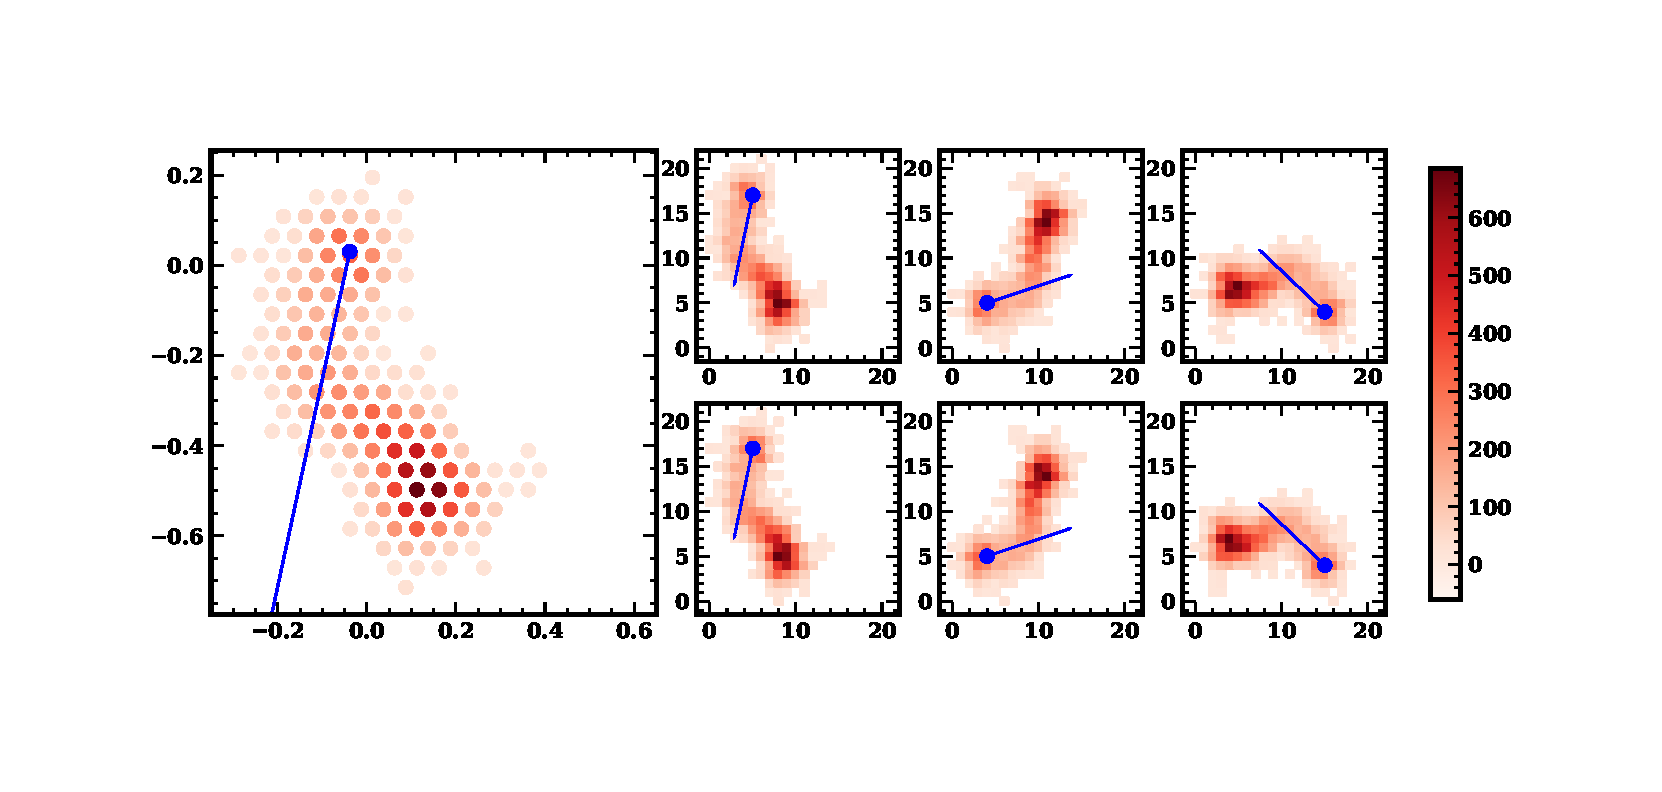
\includegraphics[width=1.05\textwidth]{figures/fig2.pdf}
% \captionsetup{justification=centering,skip=2pt,font=scriptsize}
\caption{Example square conversions of a 6.4 keV hexagonal track (left panel). The six panels to the right show shifts along the 120$^\circ$ GPD axes; shifting odd rows (upper) or even rows (lower). For each hexagonal track, CNNs are fed column-wise pairs of square conversions, along with the energy, absorption point (blue dot) and initial photoelectron direction (blue line) as labels.}
\label{fig:square}
\end{figure}

\section{Geometric bias}
\label{sec:geom}
Imaging polarimeters like IXPE use hexagonal pixels for two reasons: 
\begin{enumerate}
    \item Hexagonal arrays are the densest possible 2D packing, meaning more pixels per unit area thus improved track resolution.
    \item Hexapolar grid effects are orthogonal to the quadrupolar polarization signal. 
\end{enumerate}
The discrete nature of the pixel grid means that track elongations and emission directions are better resolved along some axes of symmetry than others, potentially creating preferred directions for reconstruction. This bias would only be visible when the pixel size is significant compared to the track size, i.e., for small, low energy tracks.
The hexagonal grid used in the IXPE GPDs is designed to minimize any polarization systematics arising from these biases.
Although not all imaging polarimeters use hexagonal pixels, this section describes some potential neural network solutions for dealing with non-square pixels.

A hexagonal grid is not natively compatible with standard CNN implementations for square matrices. It is possible to transform from a hexagonal to a square grid, however a naive transformation can lead to polarization systematics. Polarization estimation, step 2 \S\ref{chap:sbi}, expects unbiased estimators for the emission angles. CNNs learn to prefer some emission angles over others, possibly interfering with the polarization signal.
In a naive hexagonal to square conversion, emission angle bias happens partly because the CNN convolutional kernels are not spatially equivariant in hexagonal space. A possible solution is to work directly with hexagonal convolutions \citep{steppa_hexagdly_2019}, but \citet{peirson_deep_2021} describe an expedient method.

% \begin{svgraybox}
% Unlike many machine learning problems where the aim is to simply minimize the prediction error on unseen examples, in track reconstruction prediction bias must also be minimized since strong biases break the assumptions in step 2: polarization estimation.
% \end{svgraybox}

\subsection{Hexagonal to square conversion}
It is possible to leverage existing square CNN architectures by using an appropriate polarization-systematic-free hexagonal to square conversion. From \citet{peirson_deep_2021}:
\begin{quotation}
There are two main ways of converting between hexagonal and square grids: interpolation and pixel shifting. Interpolation places a fine square grid on top of the hexagonal image and interpolates.
Interpolation should generally be avoided since it adds noise to the raw data and is not easily reversible.
%Furthermore, the square representations it produces 
Pixel shifting rearranges pixels by shifting alternate rows and then rescaling \citep{steppa_hexagdly_2019} ... To avoid any polarization bias from the conversion, we pixel shift each track along each of the six hexagonal axes. Hexagonal tracks are rotated so that rows align horizontally (this can be done in three different ways, separated by $120^{\circ}$), then alternate rows are shifted (this can be done in two different ways, left and right) so that the track resembles a rectangular grid. We convert the rectangular grid into a square image by defining the leftmost track pixel and bottom track pixel as the left edge and the base of the image respectively. A square image size of 50x50 pixels is used to fit all track sizes for energies up to 11 keV.
Since square track images are defined independently of the absolute hexagonal coordinate values, the initial hexagonal track rotation can be performed about any axis.

% The HexagDLy \citep{steppa_hexagdly_2019} software, designed for use in CTA, allows standard CNNs to operate on hexagonal images. It does this by pixel shifting the images to square arrays and then applying specialized convolutional kernels that preserve equivariance in hexagonal space. Unfortunately, in practice, this method proved too slow to train for the large event sets required for polarization estimation. 

A single hexagonal track thus produces six square conversions, fig.~\ref{fig:square}, two for each $120^{\circ}$ angle.
A single training example for the CNNs is formed by stacking the corresponding square conversion pair, similarly to color channels in a \textit{rgb} image CNN problem -- in this case with only two channels. At test time all 3 pairs are evaluated by the CNNs and the predicted angles are rotated back to their original direction. 
\end{quotation}
This approach artificially approximates spatial equivariance of CNN convolution kernels in the hexagonal space and removes all relevant prediction bias on emission angles $\theta$ (and later $p_0, \theta_0$) introduced when converting from hexagonal to square coordinates.
%This approach can cause some hexagonal systematics...


% Our hexagonal to square process is shown in algorithm~\ref{alg:hex} for an individual track, with additional details in the hexagdly documentation:
% \begin{algorithm}[]
% \SetAlgoLined
% 1:Rotate hexagonal coordinates so that the axes of symmetry are aligned with the desired square grid (this is already the case for fig.~\ref{hex},fig.~\ref{square}). The track angle vectors must be rotated in the same way. \\
% %2: Calculate the distance between hexagon centres and edges $a$, and centres and corners $r$.  \\
% 2: Shift even rows to the left by half the pixel-to-pixel distance. The pixels now form a rectangular grid. This is read out into a 2D array giving the first square image.  \\
% % 2: Shift odd rows to the left by half the pixel-to-pixel distance. This gives the first square image.  \\
% \For{$m = 1 : M$}{
% 3: }

% 4: \\
% 5: \\
% 6: 
% \caption{Pseudocode for the hexagonal track to square track conversion process.}
% \label{alg:hex}
% \end{algorithm}
% Fig.~\ref{fig:square} shows an example hex2square conversion.


\section{Deep ensemble setup} 
\label{sec:deepset}
The specific CNN model that will compose the deep ensemble has to be chosen before any training begins. CNN architectures are usually compared by their performance on natural image classification datasets, like imagenet (224x224 pixels) or CIFAR (32x32 pixels) \citep{doon_cifar-10_2018}. The residual network architecture (ResNet, \citet{he_deep_2015}) described in \S\ref{sec:CNN} and related architectures like DenseNet \citep{huang_densely_2018} became the state of the art for image processing benchmarks in 2017. \citet{peirson_deep_2021} use the ResNet-18 CNN architecture to compose the deep ensemble; this has 18 total layers. The results shown in this section are using ResNet-18s, but any DNN appropriate for images could be used. Indeed, as of 2020, transformer architectures \citep{vaswani_attention_2017} have supplanted residual networks as the latest state of the art in image processing. 

During training, each CNN minimizes a loss function. Since track reconstruction is a multitask problem, the loss function will include multiple terms for emission angle loss, absorption point loss, and energy loss. The DNNs will also predict the aleatoric uncertainty on each of its estimates. Each task loss function term is considered separately and they are all combined at the end of the section.

\subsection{Emission angles} 
Since emission angles are periodic, a Gaussian aleatoric uncertainty is inappropriate.
Instead of the Gaussian negative log-likelihood (NLL) used in \S\ref{sec:deepens}, the von Mises (VM) distribution NLL is a better loss function choice. This is the maximum entropy distribution for circular data with specified expectation. For a random 2D unit vector $\mathbf{x}$
\begin{equation}
    {\rm VM}(\mathbf{\mu},\kappa) \equiv p(\mathbf{x}|\mathbf{\mu},\kappa) = \frac{\exp (\kappa \mathbf{\mu}^T\mathbf{x})}{2\pi I_0(\kappa)}.
\end{equation}
where $I_0$ is the modified Bessel function of the first kind.
This can also be considered a 1D distribution over the polar angle $\theta$ of vector $\mathbf{x}$:
\begin{equation}
    {\rm VM}(\theta_{\mu},\kappa) \equiv p(\theta|\theta_{\mu},\kappa) = \frac{\exp (\kappa \cos(\theta - \theta_{\mu}))}{2\pi I_0(\kappa)}.
\end{equation}
The VM distribution is parameterized by concentration parameter $\kappa$; for large $\kappa$ the VM converges to a Gaussian with variance $\sigma^2 = 1/\kappa$. For small $\kappa$ the VM converges to a uniform distribution.
This more appropriately reflects the distribution of predictions $\hat{\theta}$, which are clearly periodic.

Predicting scalar periodic values directly is tricky for standard DNNs, so the emission angle $\theta$ can be parameterized as a 2D vector $\mathbf{v} = (\rm{cos}2\theta,\rm{sin}2\theta)$. Now the DNNs attempt to predict the 2D vector $\hat{\mathbf{v}}$ \citep{peirson_deep_2021}. Only $-\pi/2 \leq \hat{\theta} < \pi/2$, as opposed to $-\pi \leq \hat{\theta} < \pi$, are required for polarization estimation since the EVPA $-\pi/2 \leq \theta_0 < \pi/2$, i.e. polarization is a quadrupolar signal. However, the full $2\pi$ emission angle can be useful when dealing with systematics and extended source analysis. If predicting the full $2\pi$ emission angle is necessary, an additional loss term for $\mathbf{v}_2 = (\rm{cos}\theta,\rm{sin}\theta)$ can be included \citep{peirson_deep_2021}. Predicting only $\mathbf{v}_2$ gives very poor results for low energy tracks because of direction ambiguity, and should be avoided.

Each DNN model in the ensemble computes the emission angle loss for track image $\mathbf{x}$ with true direction $\theta$ as the VM NLL 
\begin{equation}
    L_{\theta}(\mathbf{v} \mid \mathbf{x}) = -\hat{\kappa}^a(\hat{\mathbf{v}}.\mathbf{v}) + \log I_0(\hat{\kappa}^a) .
    \label{eqn:loss}
\end{equation}
where $\hat{\kappa}^a$ are the DNN predicted aleatoric VM uncertainties.
The epistemic uncertainties can also be assumed to follow ${\rm VM}(0,\kappa^e)$; $\kappa^e$ can be estimated from the output of a deep ensemble with M DNNs $\{\hat{\theta}_{j}\}^M_{j=1}$ using the appropriate maximum likelihood estimator:
\begin{equation}
    \bar{R}^2 = \left(\frac{1}{N}\sum_{j=1}^M\cos2\hat{\theta}_{j}\right)^2 + \left(\frac{1}{N}\sum_{j=1}^M\sin2\hat{\theta}_{j}\right)^2 
\end{equation}
\begin{equation}
    \label{eqn:epis}
    \frac{I_1(\hat{\kappa}^e)}{I_0(\hat{\kappa}^e) } = \bar{R},    
\end{equation}
The total VM predictive error on each track angle $\hat{\theta}$ is approximated by summing the aleatoric and epistemic variances, as in \S\ref{sec:deepens}: 
\begin{equation}
\frac{1}{\hat{\kappa}} =   \frac{1}{\hat{\kappa}^e} + \frac{1}{M}\sum_{j=1}^M \frac{1}{\hat{\kappa}^a_{j}}
\end{equation}


\subsection{Absorption points} To predict the (x,y) photon absorption point coordinates given a track image $\mathbf{x}$, a simple Gaussian NLL loss function suffices:
\begin{equation}
     \label{eqn:DE_abs_loss}
    L_{\rm abs}(x,y \mid \mathbf{x}) = \frac{1}{2}\log\hat{\sigma}_{\rm abs}^2 + \frac{1}{2\hat{\sigma}_{\rm abs}}\bigg\|
    \begin{bmatrix}
    x \\ y
    \end{bmatrix}
    - \begin{bmatrix}
    \hat{x} \\ \hat{y}
    \end{bmatrix}\bigg\|^2.
\end{equation}
As in eq.\ref{eqn:log_loss}, the DNN actually predicts the log variance for numerical stability. If desired, the epistemic error for the absorption point predictions can be calculated in the same way as \S\ref{sec:deepens}.


\subsection{Photon energy}
Similarly to the absorption point loss eq.\ref{eqn:DE_abs_loss}, the energy loss can be stated as a simple MSE with the aleatoric error included:
\begin{equation}
     \label{eqn:Eloss}
    L_{E}(E \mid \mathbf{x}) = \frac{1}{2}\log\hat{\sigma}_E^2 + \frac{1}{2\hat{\sigma}_E}\big\|
    E
    - \hat{E}\big\|^2,
\end{equation}
and like the absorption points, the epistemic error can be calculated over the deep ensemble as in \S\ref{sec:deepens}.

Predicting the energy, while simple at first sight, is more tricky than absorption points because of tail tracks.
The presence of tail tracks, \S\ref{sec:tail}, can cause the DNNs to produce biased energy estimates $\hat{E}$ with this loss function. Tail tracks look like lower energy tracks than their true energy label suggests, and this can lead to two possibilities:
\begin{itemize}
    \item If tail tracks are difficult to distinguish from peak tracks this will cause the DNN to skew its overall predictions upward in energy to minimize eq.\ref{eqn:Eloss}.
    \item If low energy tail tracks are difficult to distinguish from high energy tail tracks, then most tail tracks will be assigned the mean energy of the training distribution as this minimizes the expected value of eq.\ref{eqn:Eloss}. This is usually undesirable for astrophysical spectra.
\end{itemize}
In principle these two effects could be remedied in a number of ways, for example by adjusting the loss function eq.\ref{eqn:Eloss} \citep{peirson_deep_2021} or by a careful look at the predicted energy uncertainty (tail tracks should have much higher uncertainties).
In practice, since tail tracks also affect emission angle reconstruction and by extension polarization estimation, the recommended approach is to remove tail tracks from the analysis to the greatest extent possible \citep{peirson_towards_2021}. This works well only if tail tracks are distinguishable from peak tracks. For IXPE GPD events this is fortunately the case, but a different approach may be better for other imaging X-ray polarimeters. In \S\ref{sec:removetail} we describe a DNN approach to identify and remove tail tracks. \\

The full DNN loss function to be minimized is now
\begin{equation}
\label{eqn:fullloss}
    L(\theta, x, y, E \mid  \mathbf{x}) = L_{\theta} + L_{\rm abs} + L_{E} + \alpha \|\mathbf{w}\|^2,
\end{equation}
where the final term is an L2 regularization on the DNN weights controlled by hyperparameter $\alpha$, to prevent overfitting the training data. The predicted aleatoric uncertainties act as automatically tuned hyperparameters for the remaining loss terms \citep{kendall_multi-task_2018}. Given a track image input $\mathbf{x}$, an individual DNN outputs an 8 dimensional vector: $(\hat{\mathbf{v}}, \hat{\kappa}^a,\hat{x}, \hat{y}, \hat{\sigma}_{\rm abs}, \hat{E}, \hat{\sigma}_{E})$.



\section{Removing tail tracks}
\label{sec:removetail}
Photoelectron tracks from events converting outside the main detector gas are known as tail tracks, \S\ref{sec:tail}. For both DNNs and classical methods they cause problems with photon energy prediction, discussed in \S\ref{sec:deepset}. Furthermore, tail tracks have comparatively high emission angle prediction error (low polarization sensitivity \S\ref{sec:tail}) and \S\ref{sec:perform} will show that this error is not properly captured by deep ensemble predictive uncertainties. One possible approach to remedy the tail track issue is to attempt to excise tail tracks from the data analysis entirely.     

\begin{figure}[t]
\centering
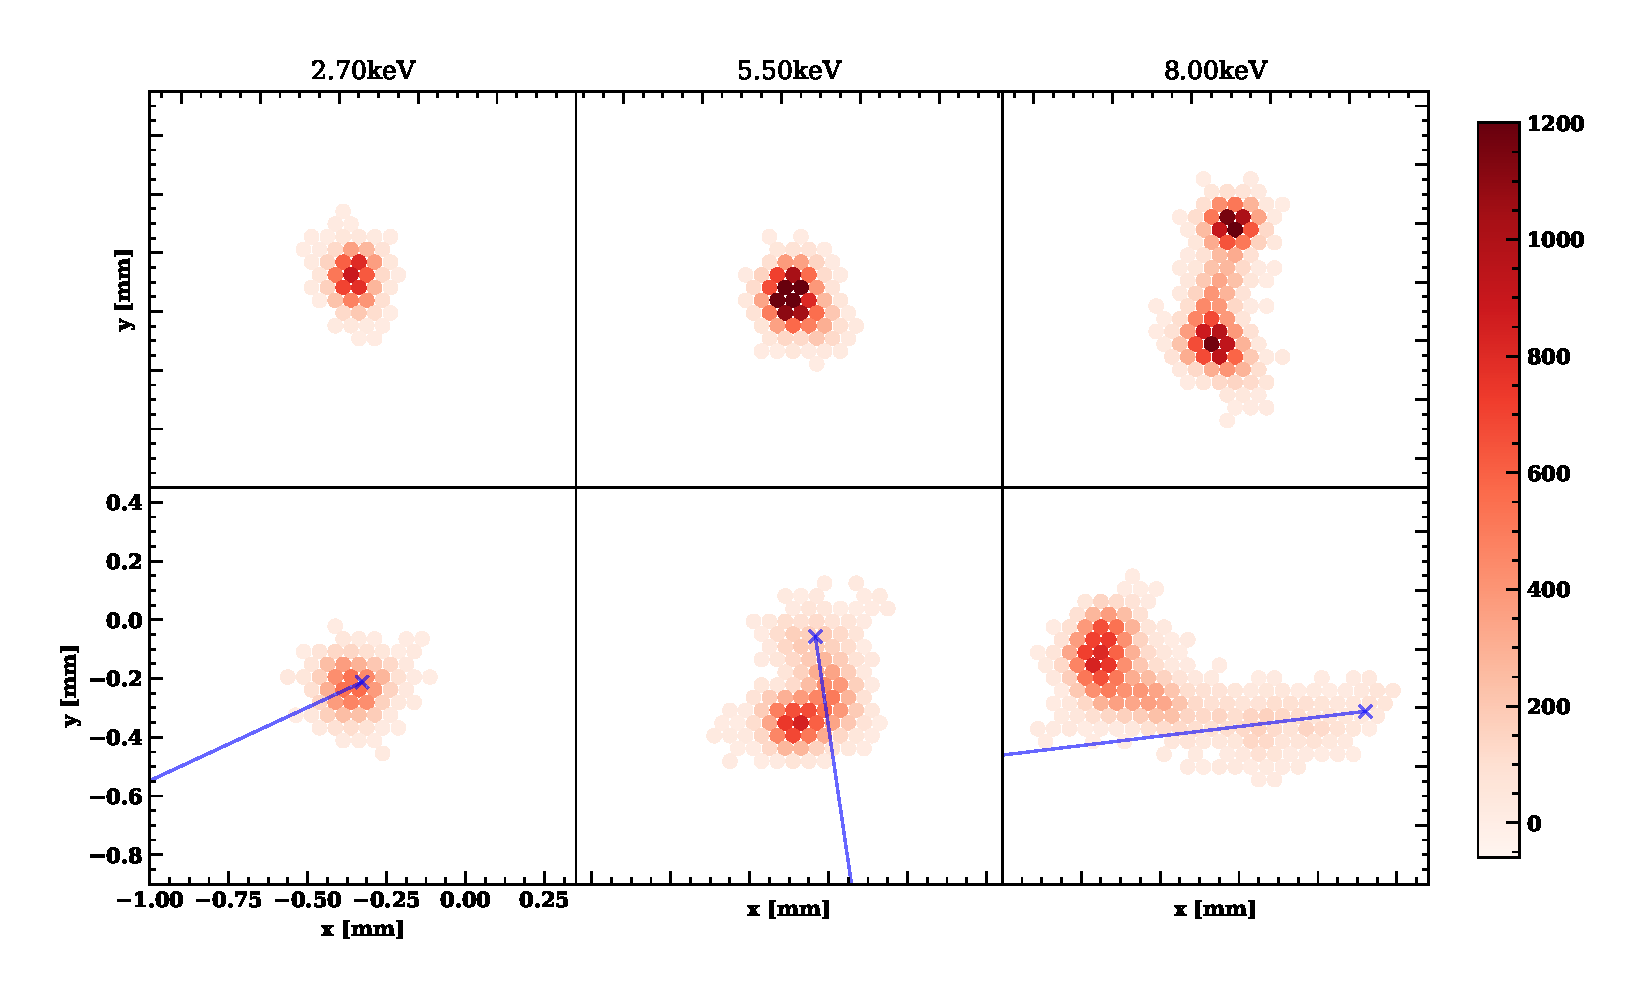
\includegraphics[width=1.05\textwidth]{figures/fig4.pdf}
% \captionsetup{justification=centering,skip=2pt,font=scriptsize}
\caption{Example tail events (top row) and peak events (bottom row) for three different recovered energies. All plots follow the same spatial and color scale. These tail events convert in the GEM. Color denotes charge deposited in a given detector pixel. Note that tail events are more compact, short and with high charge density at maximum.}
\label{fig:tailvpeak}
\end{figure}

For IXPE's GPDs, tail tracks differ in morphology from peak events converting in the gas. Fig.~\ref{fig:tailvpeak} compares events with the same linearly recovered energy (largely determined through the summed pixel counts, the summed energy deposition in the gas). Since the GEM and window material have a lower mean free path for photoelectrons, detected tail events are typically due to photo-electrons ejected close to the GEM/window normal. Their tracks are thus more compact, with higher counts/pixel for the same recovered energy. Window events have larger drift diffusion than GEM conversions. Distinguishing peak and tail tracks can be formed as a computer vision classification problem, so a DNN would be a good model choice and could be trained on simulated events to recognize the differences. 

A good approach for peak vs. tail track classification would be to include the classification task into the existing track reconstruction deep ensemble, \S\ref{sec:deepset}. This would likely improve performance over training a separate model and at first glance would only require an additional loss term in eq.\ref{eqn:fullloss}. However, this approach would not fix the problem of improper energy predictions and emission angle uncertainties unless more complex cross terms to eq.\ref{eqn:fullloss} were also added. The cross terms would ensure, for example, that tracks likely to be tail events have higher energy uncertainty. Opting for a simpler approach, \citet{peirson_towards_2021} trained a separate peak vs. tail classifier DNN and used only peak tracks to train the track reconstruction deep ensemble. The \citet{peirson_towards_2021} separation approach is described in this section, but a unified deep ensemble approach to tail vs peak classification would likely work better and is discussed as a future direction in \S\ref{chap:conc}.
%also treating GEM tails and window tails separately would also improve things.

\begin{figure}[t]
\centering
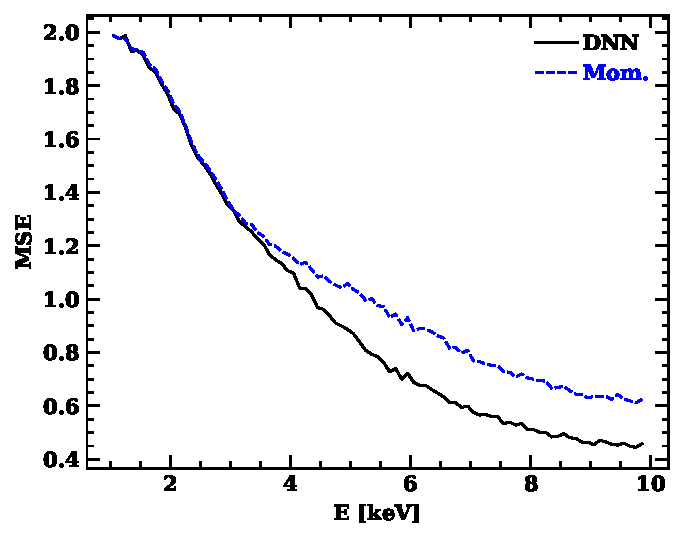
\includegraphics[scale=.75]{figures/mse.pdf}
\caption{Mean squared error on emission angle prediction as a function of photon energy, measured using eq.~\ref{eqn:vmse}, for the classical moment analysis and deep ensemble.}
\label{fig:mse}      
\end{figure}

Setting up a peak vs. tail DNN classification model is the same as setting up a multitask deep ensemble \S\ref{sec:deepset}, only now the loss function to be minimized is different. In binary classification tasks, DNNs minimize the cross-entropy loss, eq.\ref{eqn:eglossbin}.
Given a single input, a DNN outputs a single scalar between 0 and 1 that represents the probability an input is the first class. \citet{peirson_towards_2021} use exactly the same ResNet-18 architecture and data preprocessing, \S\ref{sec:data}--\ref{sec:geom}, when training the peak vs. tail classifier DNN; the only notable differences are the loss function and data labels.
%deep ensemble?


\section{Training and ensemble selection}
\label{sec:trainens}
Individual DNN training procedures should follow the guidelines in \S\ref{sec:training}, \S\ref{sec:val}. Specifics will depend on the particular DNN architecture chosen. CNNs for computer vision problems train particularly well using stochastic gradient descent with momentum \citep{sutskever_importance_2013} as the optimization algorithm. Normalizing the inputs and outputs before training typically helps improve convergence. From \citet{peirson_deep_2021}:
\begin{quotation}
The ResNet-18 architecture trains in a reasonable amount of time ($\sim 15$ hours for 150 epochs on 4 Nvidia Titan GPUs, using a batch size of 2048). 
Before training, we normalize the track images, subtracting the pixel-wise mean from each track image and dividing by the pixel-wise standard deviation (where the mean and standard deviation are calculated over the full training set). The track energy and absorption point labels are similarly processed.
Normalizing the training data helps prevent vanishing and exploding gradients during the NN training procedure and lead to faster convergence. We use stochastic gradient descent with momentum as our optimizing algorithm, typical in computer vision tasks \citep{sutskever_importance_2013}, with a stepped decaying learning rate starting at 0.01.
We choose batch sizes of 512, 1024, 2048 tracks ... We tune the hyperparameters to minimize the MSE for the validation set.
\end{quotation}
Once multiple DNNs are trained with optimized hyperparameters, individual DNNs should be chosen at random to compose the ensemble. This ensures accurate epistemic uncertainty estimates.

\begin{figure}[t]
\centering
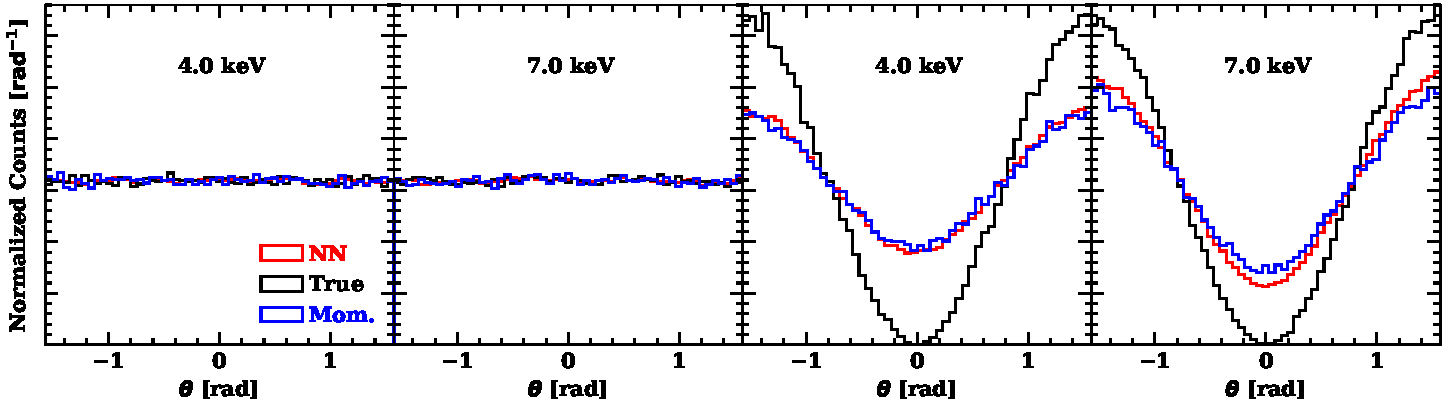
\includegraphics[width=1.0\textwidth]{figures/angle_flat.pdf}
% \captionsetup{justification=centering,skip=2pt,font=scriptsize}
\caption{Emission angle recovery for unpolarized, $p_0 = 0$, (left two panels) and 100\% polarized, $p_0 = 1$, (right two panels) simulated IXPE data for $4.0$ and $7.0$\,keV. The true photoelectron angle distribution is shown in black; standard moment analysis reconstruction is in blue and deep ensemble in red.}
\label{fig:angledist}
\end{figure}

\section{Performance}
\label{sec:perform}
The performance of deep ensembles in track reconstruction is compared to the classical moment analysis \S\ref{chap:intro} on simulated IXPE data. The results shown are for peak events only unless otherwise specified.


\subsection{Emission angles}  Two important measures of performance should be evaluated for emission angle recovery: the accuracy of recovery and the quality of uncertainty estimates. The accuracy of emission angle recovery can be measured, for example, by the MSE on a test dataset
\begin{equation}
\label{eqn:vmse}
    \frac{1}{N}\sum^N_{i=1} \|\mathbf{v}_i - \mathbf{\hat{v}}_i\|^2.
\end{equation}
Fig.~\ref{fig:mse} gives the above MSE as a function of the true track energy on an unpolarized IXPE test dataset for both classical moment analysis and deep ensemble approaches. At low energies, deep ensembles fail to improve significantly over the moment analysis; when resolution is low, track image moments contain all the relevant information. 

It is also essential to confirm that the estimates $\hat{\theta}$ are unbiased.
Fig.\ref{fig:angledist} gives the distribution of emission angles $\hat{\theta}$ recovered by the deep ensemble and moment analysis for an unpolarized and polarized source at various energies. For both methods, emission angle estimates show no systematic biases, and at higher energies for the polarized source the improved signal recovery of the deep ensemble is visible. 
As an additional check, the bottom row of fig.~\ref{fig:kappa} displays the distribution of $\hat{\theta} - \theta$ for the moment analysis and deep ensemble at three different true energies. Both the moment analysis and deep ensemble have symmetric error distributions centered at zero for all energies. At higher energies, the lower dispersion and thus higher accuracy of the deep ensemble is again clear.
%Need a plot of unbiasedness as a function of angle

\begin{figure}
\centering
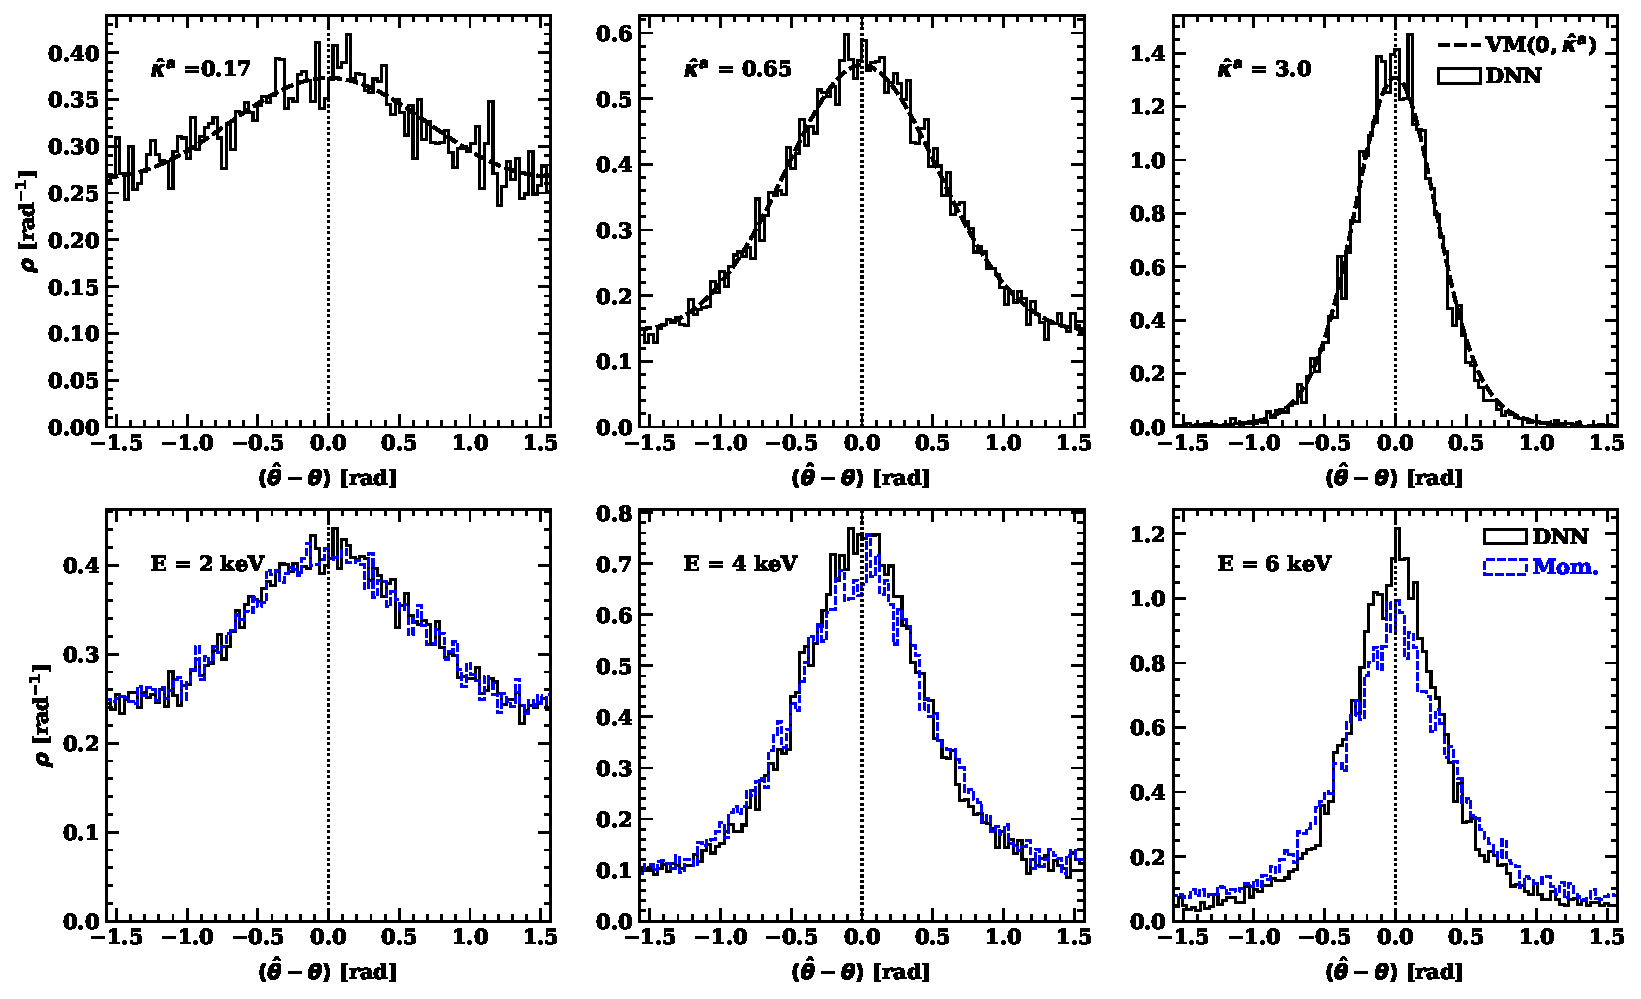
\includegraphics[width=1.0\textwidth]{figures/kappa.pdf}
% \captionsetup{justification=centering,skip=2pt,font=scriptsize}
\caption{\textit{Top:} Histograms of the DNN emission angle residual for three different DNN predicted aleatoric VM concentration parameters $\hat{\kappa}^{a}$. The DNN predicted VM error distributions are over-plotted. The DNN is able to correctly predict its emission angle aleatoric error distribution. \textit{Bottom:} Histograms of emission angle residuals at three different energies for DNNs and the moment analysis. All methods are unbiased (centered at zero) and at higher energies the DNNs have better recovery of the true emission angle $\theta$, as evidenced by the larger peak heights.}
\label{fig:kappa}
\end{figure}
% As usual (reading left to right) I's prefer the moments in the left panel and the N in the middle.

\begin{figure}
\centering
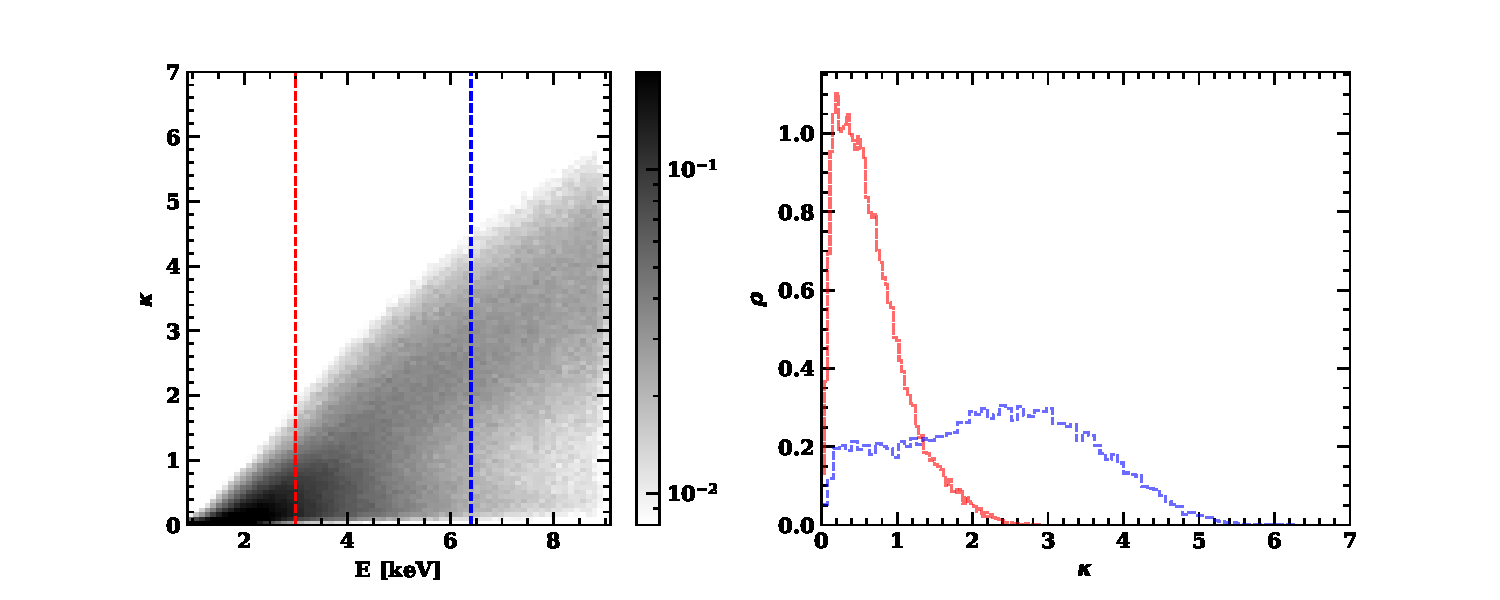
\includegraphics[width=1.05\textwidth]{figures/kappa_dist.pdf}
% \captionsetup{justification=centering,skip=2pt,font=scriptsize}
\caption{Distribution of deep ensemble predicted concentration parameters $\hat{\kappa}$ across the IXPE energy spectrum (left). The right-hand plot shows the $\hat{\kappa}$ distribution for two specific energies $3.0$ keV (red), $6.4$ keV (blue). High concentration parameter $\kappa$ means a low predictive uncertainty.}
\label{fig:kappadist}
\end{figure}

A simple way to assess the deep ensemble predicted uncertainty estimates $\hat{\kappa}$ is to consider the distribution of $\hat{\theta} - \theta$ for fixed $\hat{\kappa}$. According to the assumptions in \S\ref{sec:deepset}, $\hat{\theta} - \theta$ should follow a VM(0,$\hat{\kappa}$) if the DNNs have been properly trained. In the top row of fig.~\ref{fig:kappa}, the distributions of $\hat{\theta} - \theta$ for three different fixed $\hat{\kappa}$ are displayed with VM(0,$\hat{\kappa}$) overlayed. In all cases, the distributions match very closely. Epistemic errors are negligible for the vast majority of peak tracks, suggesting good model choice and training convergence.

It is also instructive to visualize the distribution of deep ensemble predicted uncertainties as a function of energy, fig.~\ref{fig:kappadist}. For higher energies a wider range of concentration parameters are predicted and the $\hat{\kappa}$ peak moves progressively higher. Below 2keV, barely any polarization signal is recoverable with IXPE. Fig.~\ref{fig:kappadist} highlights the strong heteroskedasticity in imaging X-ray polarimetry.

\begin{figure}[b]
\centering
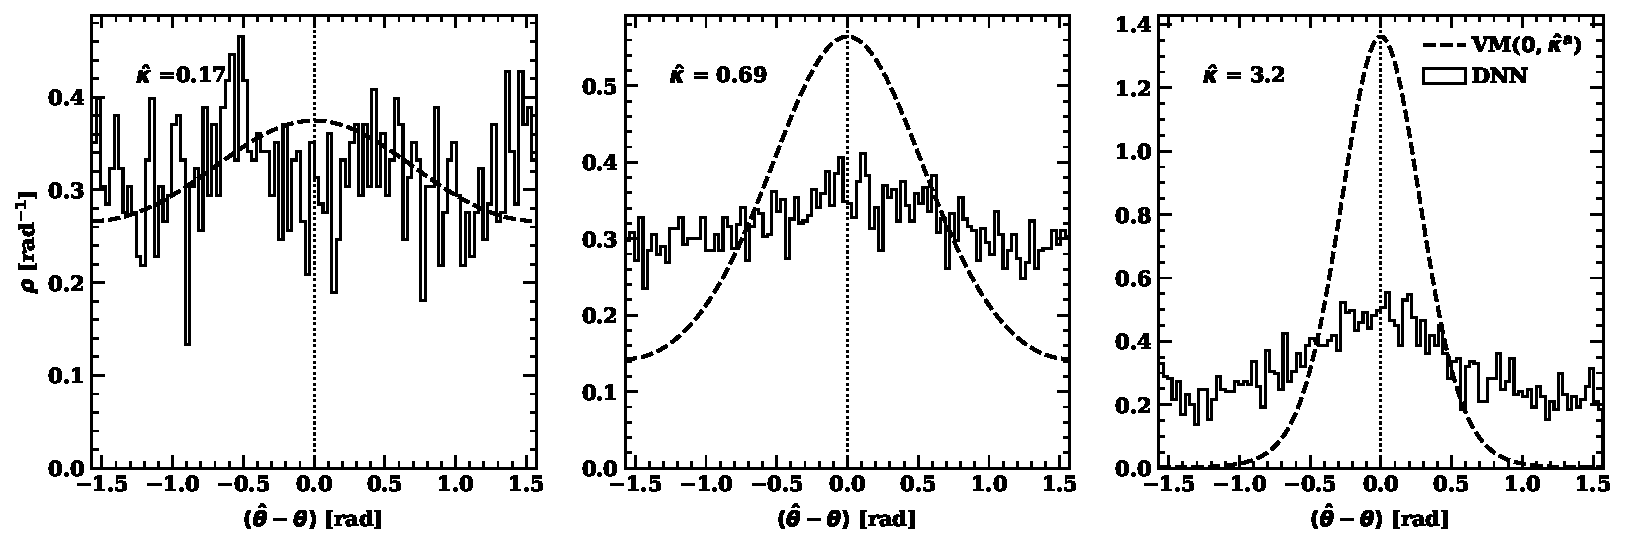
\includegraphics[width=1.0\textwidth]{figures/kappa_tail.pdf}
% \captionsetup{justification=centering,skip=2pt,font=scriptsize}
\caption{Histograms of the emission angle residual at three different DNN predicted concentration parameters $\hat{\kappa}$ for tail events only. The predicted DNN error distributions are overplotted. When tail events are treated as if they were normal events, the DNNs do not learn to predict the appropriate uncertainties.}
\label{fig:kappa_tail}
\end{figure}

For a deep ensemble trained on both peak and tail tracks, the predicted uncertainties for tail tracks are untrustworthy. Comparing the error distributions in fig.~\ref{fig:kappa_tail} to \ref{fig:kappa}, tail track error is not captured by deep ensemble uncertainty predictions, even with the epistemic uncertainty included. Furthermore, at low energies, tail track emission angle estimates are potentially biased.

\subsection{Tail vs. peak classification} For tail vs. peak classification, there is no equivalent classical method to compare the DNN performance, so this section lists the classification results achieved by \citet{peirson_towards_2021}. They use the predicted tail probability as an event threshold cut. Fig.~\ref{fig:tailcut} shows the effectiveness of different tail probability cuts. If all events with a DNN predicted tail probability higher than 70\% are removed, a loss of only 3\% of true peak events is incurred while 66\% of true tail events are successfully removed. Using a DNN classifier, only a small loss to signal events need be incurred to remove the majority of harmful tail events. Fig.~\ref{fig:tailcut} also shows how remaining tail and peak events are distributed in terms of true energy after a tail probability threshold cut. Remaining tail events come from all energies in proportion to their original population, while misidentified peak events come from middle energies where peak and tail events overlap most.

\begin{figure}[t]
\centering
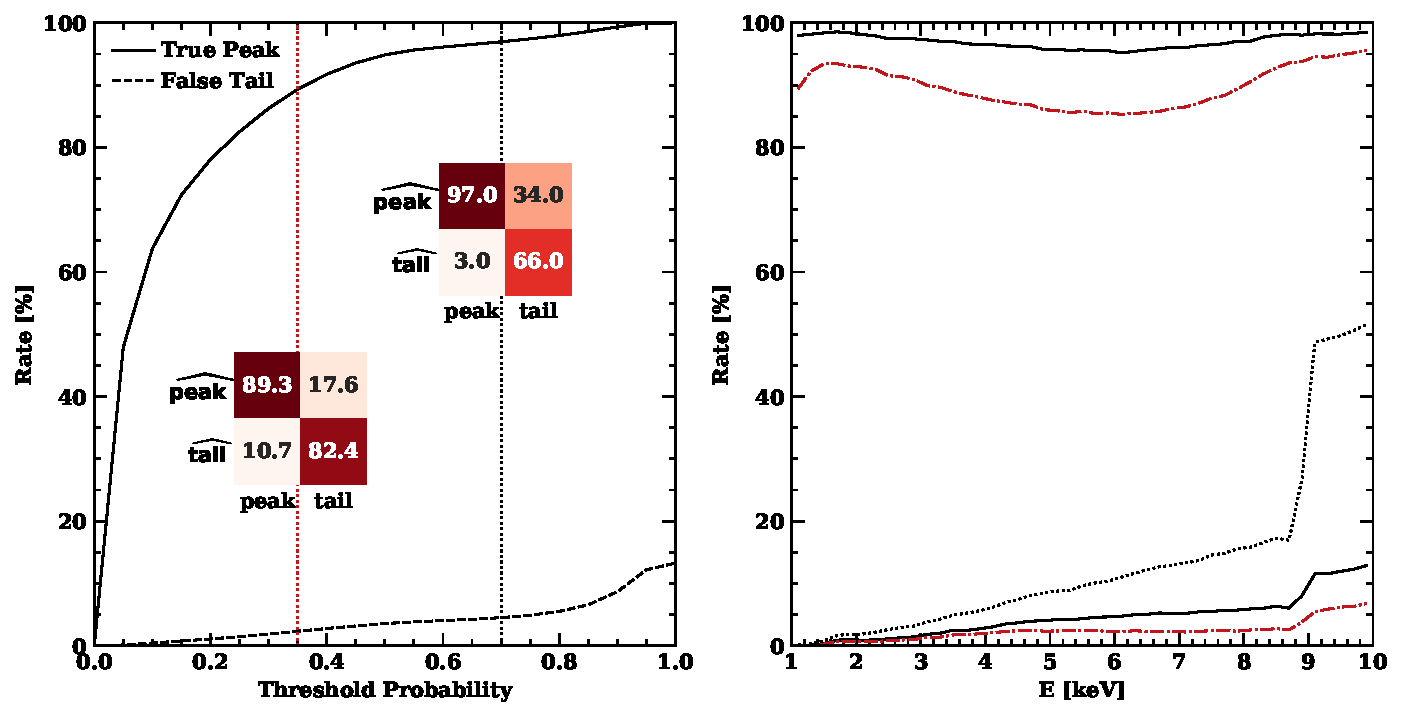
\includegraphics[width=1.0\textwidth]{figures/fig5.pdf}
% \captionsetup{justification=centering,skip=2pt,font=scriptsize}
\caption{\textit{Left:} The solid curve shows the fraction of peak events retained as a function of the tail probability cut, while the dashed curve shows the fraction of the cut sample from the remaining tail events. Insets show the confusion matrices, normalized by column, for our adopted 70\% cut and a 35\% cut. \textit{Right:} The top curves show the peak retention as a function of energy (black solid -- 70\% cut, red dot-dash -- 35\% cut). Below, the dotted curve shows the uncut fraction of the sample due to tail events, while the lower black and red curves show the residual tail pollution (70\% and 35\% cut, respectively). Depending on how harmful tail events are to the desired measurements, different cut levels could be appropriate.}
\label{fig:tailcut}
\end{figure}

At least for IXPE GPDs, it is certainly possible to meaningfully distinguish between tail and peak events. 
The upcoming section on photon energy recovery and \S\ref{chap:sbi} demonstrate how tail cuts based on DNN probabilities can be used to improve energy and polarization resolution.


\subsection{Absorption points} 
Absorption point accuracy can be evaluated using the MSE. In fig.~\ref{fig:abspts} the classical moment analysis and deep ensemble predictions are compared at different photon energies. For IXPE, the track barycenter provides a better prediction of the absorption point for very low energies -- the deep ensemble recovers this transition while the moment analysis does not. 

For current generation X-ray polarimeters like IXPE, the telescope PSF is much larger than any absorption point discrepancy, so absorption point accuracy is less essential than emission angle or photon energy accuracy. However, future missions with higher spatial resolution may require very accurate absorption point estimates for detailed imaging of extended sources.

\begin{figure}[t]
\centering
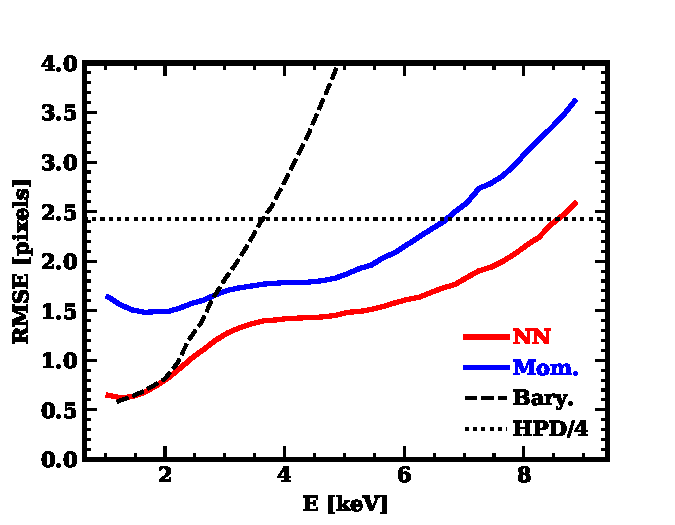
\includegraphics[scale=.65]{figures/fig8_1.pdf}
\caption{Photon absorption point localization accuracy using the root mean squared error. The deep ensemble predictions (red) do appreciably better than the moment analysis and matches a barycenter estimate at the lowest energies. For IXPE, all methods are adequate, as localization is much better than the size of the point source image produced by IXPE's mirrors. One quarter of IXPE's half power diameter is illustrated (black dotted line).}
\label{fig:abspts}       % Give a unique label
\end{figure}


\subsection{Photon energy} Energy recovery can be adversely affected by tail events. While the MSE in predicted energy is lower for deep ensemble methods compared to classical linear charge recovery, these results should be treated with caution. Much of this improvement is specious, coming from a mistreatment of tail events.
Fig.\ref{fig:energy_hist} plots the IXPE recovered energy histograms of the classical linear method (blue), a deep ensemble trained including tail events (black) and a deep ensemble trained on only peak events with tail events removed at a 70\% peak vs. tail classifier probability (red). Around the true energy peak all methods perform similarly, with a slight advantage for the DNN based methods. As the energy increases, all methods show a low energy tail in reconstructed energy which is produced by tail events. The standard deep ensemble that does not differentiate peak and tail tracks also shows a high energy tail in reconstructed energy. This tail arises from low energy peak events 'looking' like higher energy tail events, so pushing some events up to higher energy tends to minimize the MSE. As discussed in \S\ref{sec:deepset}, high energy tails in reconstructed energy are undesirable for astrophysical spectra. Training a deep ensemble with only peak events prevents this high-energy tail behavior.

Cutting events based on the predictions of the peak vs. tail classifier successfully reduces tails in the recovered energy histograms. A tail event cut improves the energy resolution at the cost of potentially losing some peak events and thus some polarization signal. \S\ref{sec:perform2} will discuss and quantify the polarization signal loss due to tail event cuts. 

The energy prediction accuracies (mean absolute error and FWHM) for all three methods as a function of photon energy are given in fig.~\ref{fig:energy_mse}. Removing tail events provides a significant improvement to the energy prediction accuracy.


\begin{figure}[t]
\centering
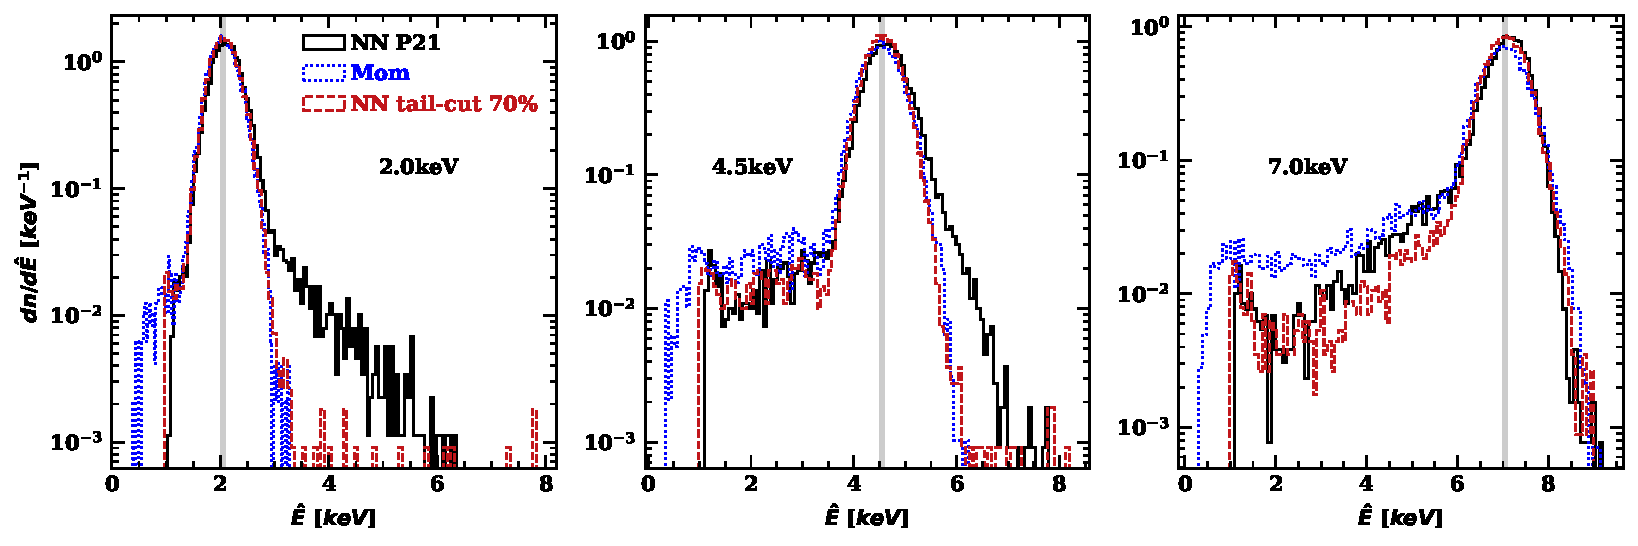
\includegraphics[width=1.0\textwidth]{figures/fig6.pdf}
% \captionsetup{justification=centering,skip=2pt,font=scriptsize}
\caption{Response for three true energies. Note that while the P21 analysis suppressed the large tail rate seen in the Moments processing, events leaked to a high energy tail for medium to low true energies. Our morphological tail cut further suppresses the GEM/window tail, avoids the high energy leakage and achieves comparable or better peak width.}
\label{fig:energy_hist}
\end{figure}

\begin{figure}[t]
\centering
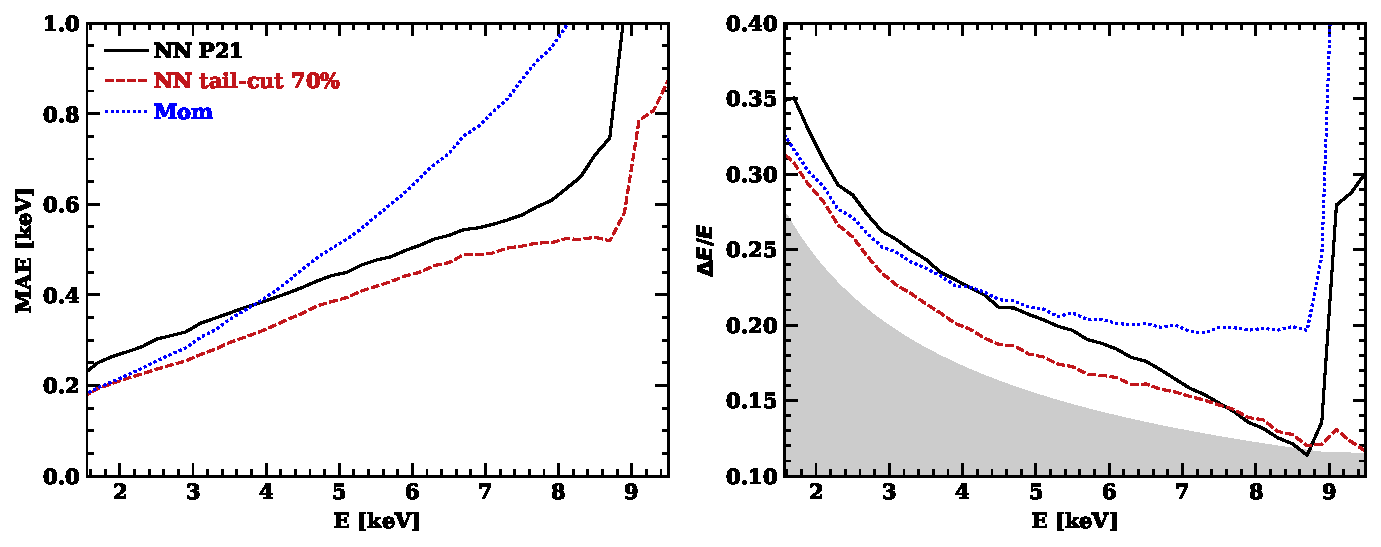
\includegraphics[width=1.0\textwidth]{figures/fig7.pdf}
% \captionsetup{justification=centering,skip=2pt,font=scriptsize}
\caption{\textit{Left:} Mean absolute error in predicted energy as a function of true energy. \textit{Right:} FWHM (3.46$\times$ Median Absolute Deviation) of predicted energy distribution for a source at energy E. The grey band marks the limiting energy resolution in the purely-exponential multiplication regime. NNs with 70\% tail cut performs better on every metric, more accurate per track and tighter resolution at all energies. All methods suffer from the large increase of tail events above 9\,keV.}
\label{fig:energy_mse}
\end{figure}
